\section{Project Team}\label{sec:team}

\subsubsection*{Björn Kirschner}
%
\begin{minipage}{0.2\textwidth}
\begin{flushleft}
	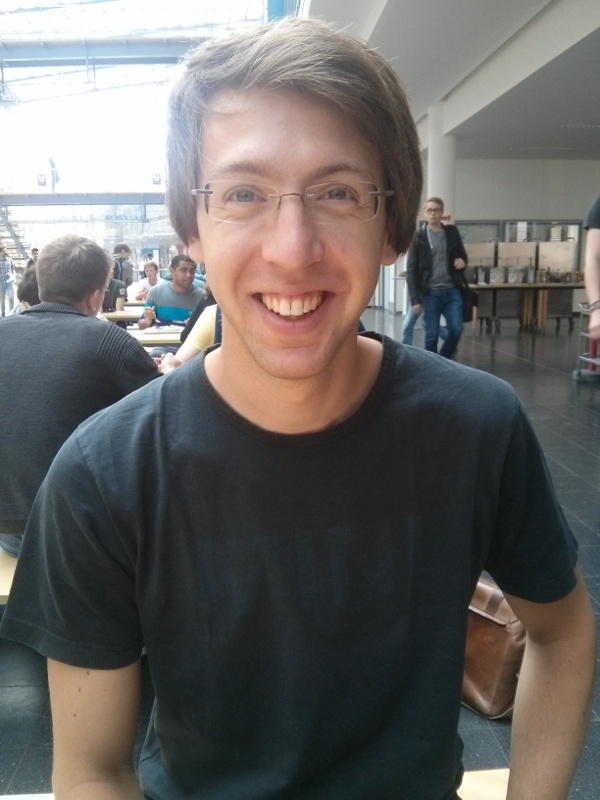
\includegraphics[width=2.2cm]{img_bjoern_small.jpg}
\end{flushleft}
\end{minipage}
\hfill
\begin{minipage}{0.8\textwidth}
%
Graduated in Information Systems at TU München. Is currently studying Information Sciences with a focus on IT security. Hence, secure communication and protocol design of the door access solution proposed in this paper will be of particular interest to him.
%
\end{minipage}


\subsubsection*{Sebastian Schleemilch}
%
\begin{minipage}{0.2\textwidth}
\begin{flushleft}
	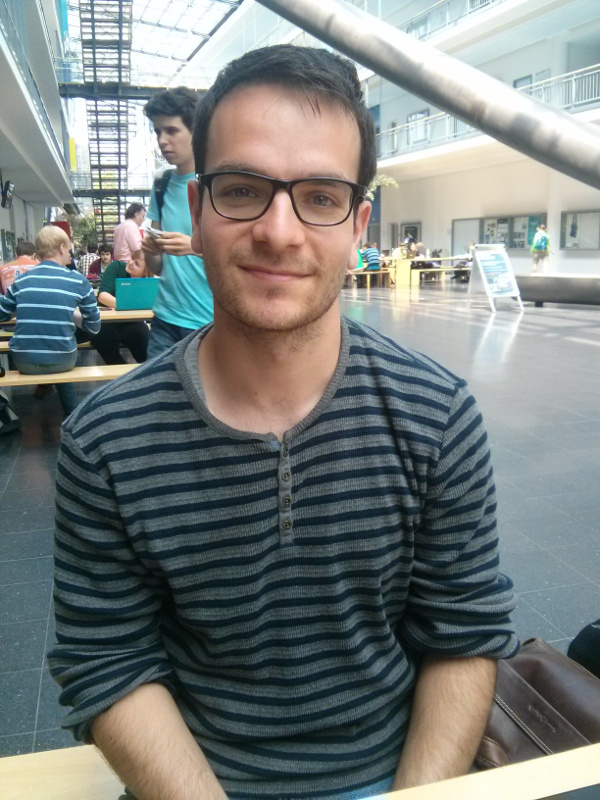
\includegraphics[width=2.2cm]{img_sebastian_small.jpg}
\end{flushleft}
\end{minipage}
\hfill
\begin{minipage}{0.8\textwidth}
%
Made his bachelor in Mechatronics at the FAU Erlangen-Nuremberg. Right now, he is studying Automotive Software Engineering at TUM in the third out of four semester. He is excited about the combination of software and the interaction with physical problems, which also explains his previous education steps so far.
Since this project will also be a mixture of pure software problems and the physical frontend (in this case: opening the door), Sebastian fits quite well into it.
%Therefore he fits quite good into the project, cause it also will be a mixture of pure software problems and the physical frontend, in this case, opening the door.
%
\end{minipage}


\subsubsection*{Stefan Smarzly}
%
\begin{minipage}{0.2\textwidth}
\begin{flushleft}
	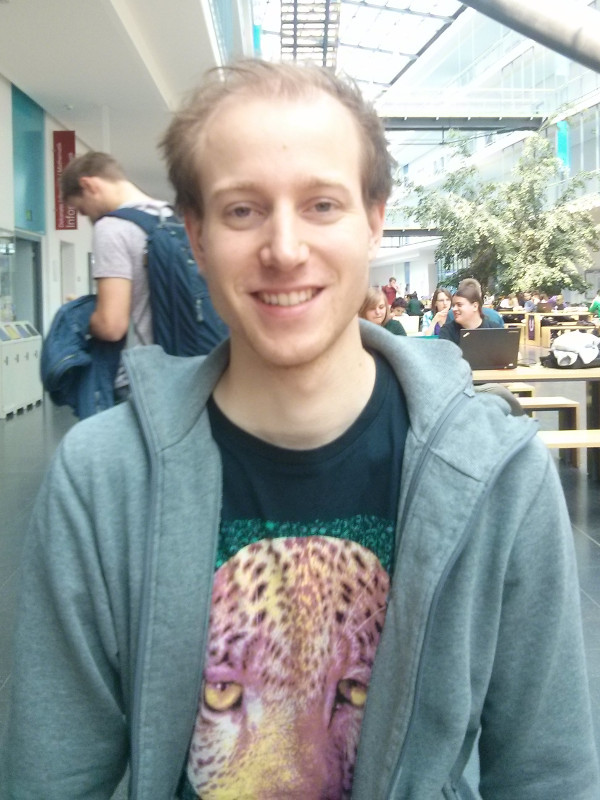
\includegraphics[width=2.2cm]{img_stefan_small.jpg}
\end{flushleft}
\end{minipage}
\hfill
\begin{minipage}{0.8\textwidth}
%
Graduated in Informatics at TU München. Currently, Stefan is studying Informatics in the Master program at TUM with an emphasis on Robotics, Distributed Networks and Security.
He is keen on working with Distributed Embedded Systems and to secure the communication between the devices.
This project provides ideal conditions to apply his knowledge about deploying a secure Distributed System that physically interacts with its environment.
%
\end{minipage}